
\chapter{Úvod do problematiky}

\section {Seznámení s biologickými pojmy}

\subsection{RNA} 

RNA (zkratka z anglického ribonucleic acid) je biomolekula, která hraje
klíčovou roli v procesu přenosu genetické informace u všech živých organismů.
RNA se skládá z řetězce nukleotidů, které obsahují cukr ribózu, fosfátovou
skupinu a jednu z pěti dusíkatých bází (adenin, guanin, cytosin, uracil nebo
inosin). Existují různé typy RNA, jako jsou messenger RNA (mRNA), ribozomální
RNA (rRNA) a transfer RNA (tRNA), které mají každý svou specifickou funkci v
buňce.

RNA sekundární struktura se týká způsobu, jakým se molekula RNA skládá na sebe
díky vzniku bázových párů mezi komplementárními nukleotidy. Bázové párování se
děje mezi dusíkatými bázemi RNA nukleotidů, přičemž adenin (A) se páruje s
uracilem (U) a guanin (G) se páruje s cytosinem (C).

RNA sekundární struktura je důležitá, protože může ovlivnit to, jak RNA
molekula funguje. Například stem-loop struktura v mRNA molekule může ovlivnit
přístupnost mRNA k ribozomům, což je buněčný mechanismus zodpovědný za
překládání mRNA na proteiny.

\section {Datové formáty}

\subsection{JSON} 

JSON (javascriptový objektový zápis) je datový formát sloužící k ukládání dat
organizovaných v polích nebo objektech. Navzdory názvu je na programovacím
jazyce nezávislý. Skládá se z dvojice klíč -- hodnota. Hodnota je libovolný
podporovaný datový typ (např.: boolean, číslo, string, pole, objekt). Níže je
úkázka JSON formátu.

\begin{code} 
{ 
  "basePairs": 
  [ 
    { 
      "basePairType": "canonical", 
      "classes": 
      [
        "bp-line" 
      ], 
      "residueIndex1": 2, 
      "residueIndex2": 118 
    } 
  ]    
} 
\end{code}

\section{Vizualizace sekundárních RNA struktur} 

Pro reprezentaci sekundární RNA struktury se používají jak textové, tak
grafické způsoby. Pro nás jsou nejzajímavějsí ty grafické, ze kterých v této
části představíme tři nejpoužívanější - linear diagram, circular diagram a
radiate diagram. Obrázky ukázek diagramu v této části jsou získané za pomoci nástroje
VARNA\cite{Varna}.

V linear diagramu jsou nukleotidy zobrazeny na rovné čáře ve stejném pořadí jako v
sekvenci a bázové páry nukleotidů jsou spojeny obloukem.

\begin{figure}[H]
  \centering
  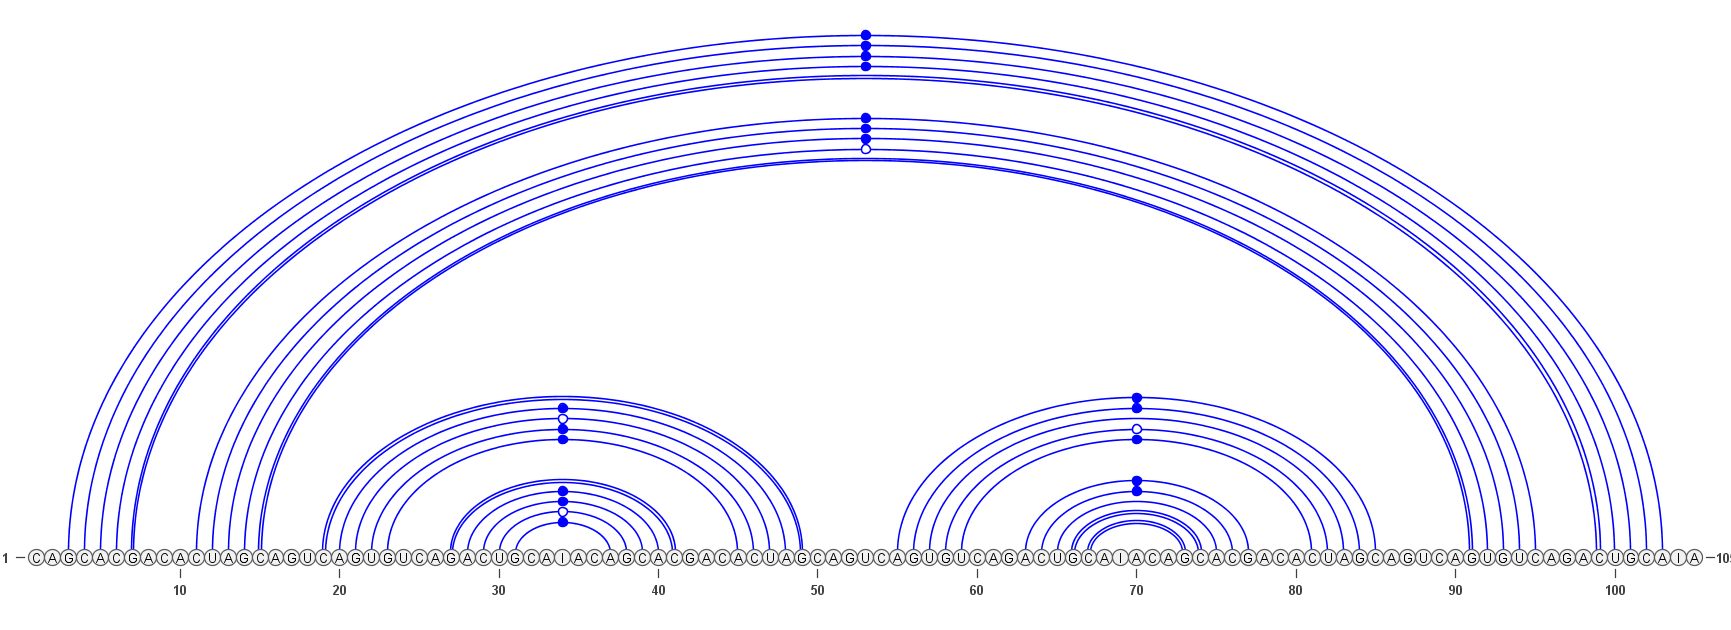
\includegraphics[width=140mm]{../img/linear.png}
  \caption{Ukázka linear diagramu}
\end{figure}

Circular diagram je velmi podobný. Nukleotidy neleží na rovné čáře, ale po
obvodu kruhu. Bázové páry jsou spojeny buď čárou nebo obloukem.

\begin{figure}[H]
  \centering
  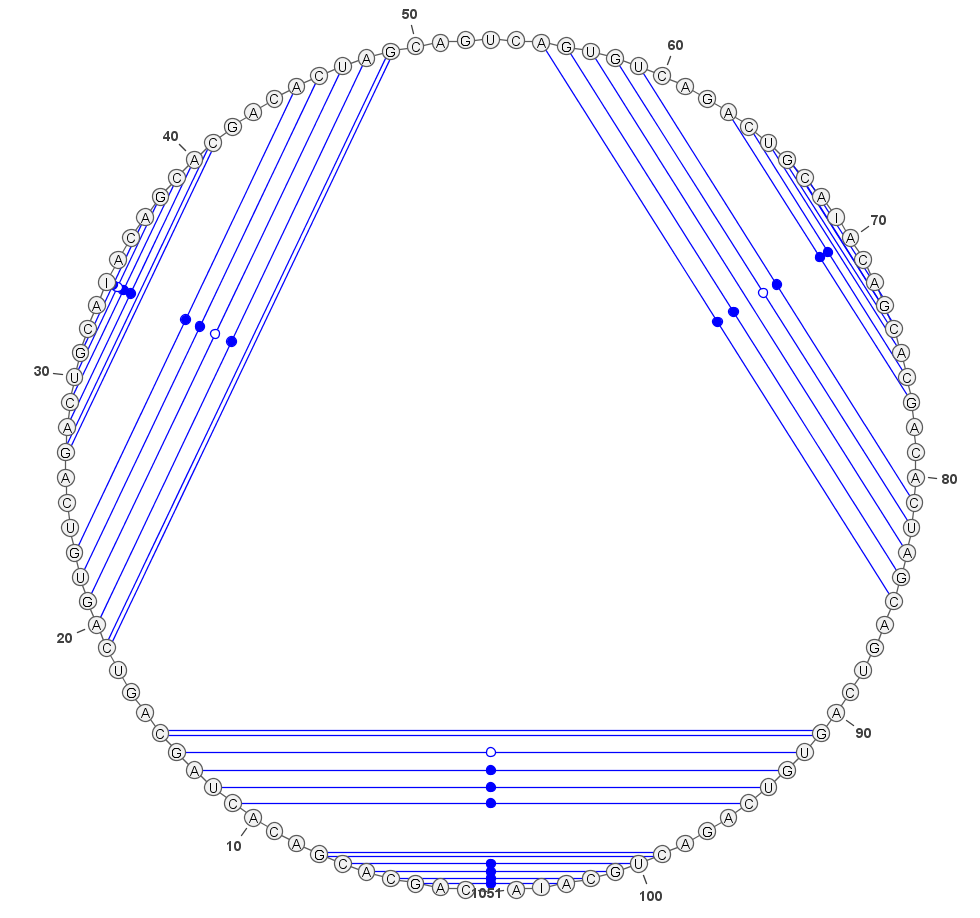
\includegraphics[height=100mm]{../img/circular.png}
  \caption{Ukázka circular diagramu}
\end{figure}

Obě tyto reprezentace postrádají schopnost zachytit motivy sekundární
struktury, a proto se radiate diagram používá tam, kde je potřeba detailní
vizuální analýza motivů sekundární RNA struktury a její interakce. V radiate
diagramu jsou pozice nukleotidů voleny tak, aby bylo možné rozeznat motivy
sekundární struktury, jako jsou hairpins, bulges nebo vícevětvené smyčky.

\begin{figure}[H]
  \centering
  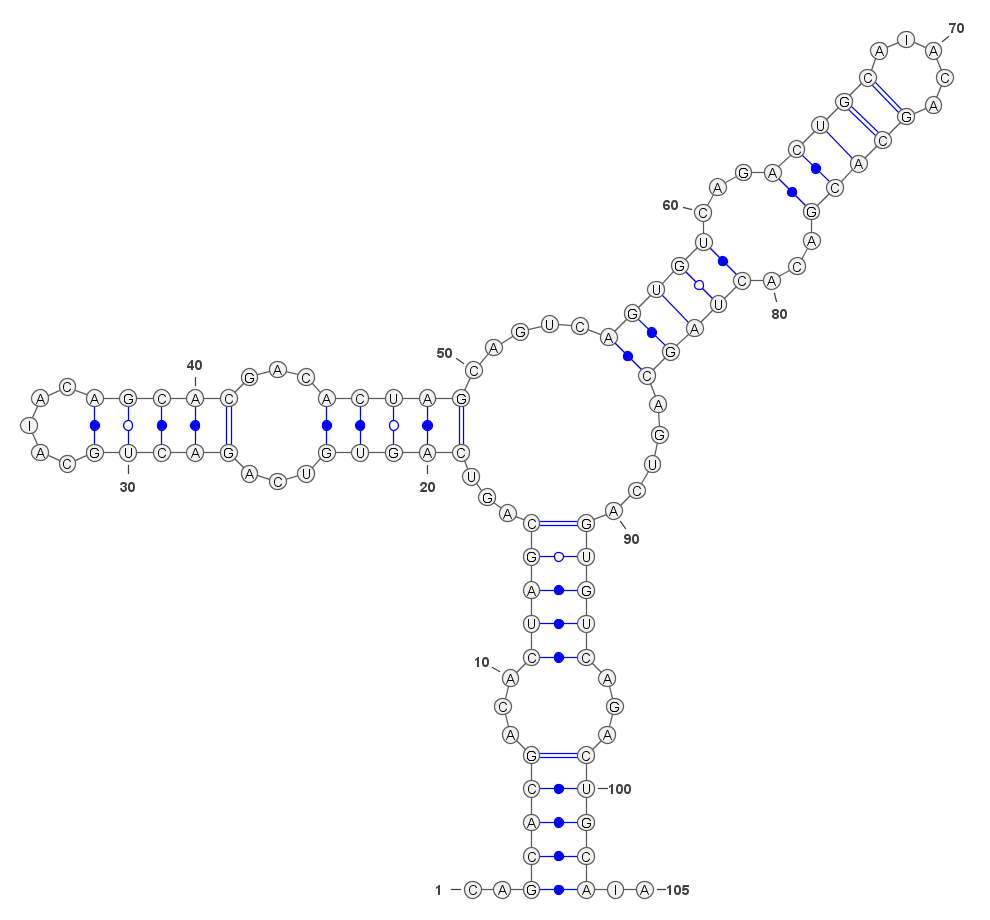
\includegraphics[height=100mm]{../img/radiate.png}
  \caption{Ukázka radiate diagramu}
\end{figure}

\section{Podobné projekty} 

Rádi bychom čtenáře seznámili s některými nástroji, které jsou používáné pro
vizualizaci sekundárních RNA struktur. Většina z nich jsou programy s
uživatelským rozhraním a mohlo by se proto zdát zbytečné je zmiňovat nebo
porovnávat s naší knihovnou. Nicméně u níže zmíněných programů není duležité
řešení samotného uživatelského rozhraní, jako především druh zvolených metod
pro vizualizaci a následné porovnávání.

Z velkého množství existujících nástrojů, byla snaha vybrat takové,
které mají rozdílné přístupy a nabízí nejširší paletu funkcí.

\subsection{VARNA} 

VARNA (Visualization Applet for RNA) je nástroj pro automatické
kreslení, vizualizaci a anotaci sekundárních RNA struktur, navržený jako
doprovodný software pro webové servery a databáze.

VARNA implementuje čtyři kreslící algoritmy, podporuje různé textové formáty
pro vstup i výstup a je schopný exportovat kresbu do rastrových nebo
vektorových formátů. Umožňuje ruční úpravy a strukturální anotace výsledku
kresby a je považován za standard pro práci se sekundárními strukturami RNA.

\subsection{RNAStructViz} 

RNAStructViz\cite{RnaStructViz} je grafický nástroj pro analýzu sekundárních
RNA struktur. Jeho předností je vizuální porovnání tří konfigurací v kompaktním
a standartizovaném circular arc diagramu. Doplněné zabudovaným prohlížečem
CT-style souboru a prohlížečem radial diagramu podstruktury, která je přímo
propojená s arc diagram oknem skrze nástroj pro výběr zoom. Mezi další funkce
patří vypočítání číselných informací a možnost exportu obrázků a dat pro
pozdější použití.

\subsection{Forna} 

Forna\cite{Forna} (force-directed rna) nabízí webové rozhraní a server, který
umožňuje uživateli vložit sekundární RNA strukturu ve formátu dot-bracket a
zobrazí ji jako force-directed
graf\footnote{https://cs.brown.edu/people/rtamassi/gdhandbook/chapters/force-directed.pdf}.
Uživatel může následně upravit pozice přetažením myší a lze i upravovat přímo
strukturu. 

\subsection{R-chie} 

R-chie \cite{Rchie} je web server, který umí vygenerovat šest různých typů arc
diagramu. Vývoj tohoto nástroje byl se zaměřením především na složitější
struktury, které nelze hezky nakreslit v radial diagramu. R-chie umí
vygenerovat diagram pro porovnávání dvou sekundárních RNA struktur. Důležitým
cílem byla možnost generovat diagramy pro velké množství dat, proto také
nenabízí grafické rozhraní a s ním spojenou interakci se strukturami. 

Projekt také nabízí balíček napsaný v jazyce
R\footnote{https://www.r-project.org/} zvaný R4RNA, který umožňuje spuštění
programu lokálně a napříč operačním systémům.

\subsection{Shrnutí existujících nástrojů}

Nástroje představené v této kapitole se soustředí především na prácí s circular
diagramem nebo linear diagramem, a právě pouze pro tyto diagramy nabízí nějaké
metody pro porovnávání omezeného množství sekundárních struktur RNA. Forna
podporuje pouze radial diagram, ale porovnávání dvou struktur, které sice jdou
zobrazit vedle sebe, už nijak neusnadňuje. 

Varna Podporuje všechny tři zmíněné diagrami, ale nelze ani zobrazit dvě
sekundární rna struktury vedle sebe. Velkou výhodou nástroje VARNA by byla
možnost použití na webu, ale k tomu používá Java Applets
\footnote{https://docs.oracle.com/javase/tutorial/deployment/applet/index.html},
které jsou od roku 2017 považované za zastaralé
\footnote{https://www.oracle.com/java/technologies/javase/9-deprecated-features.html}.

Za nejpodobnější projekt bychom považovali R-chie, který se snaží usnadnit
porovnávání sekundárních RNA struktur a nabízí i knihovnu napsanou v jazyce R.
Liší se pak v samotném přístupu, protože jejich rozhraní generuje pouze
statické circular nebo linear diagramy.

\section{Příbuzné projekty} 

Níže jsou zmíněné dva projekty, které úzce souvisí s naší knihovnou, protože
produkují data ve formátu, se kterým pracuje naše knihovna a metody
použité ke generovaní takových dat jsou klíčové pro naší knihovnu.

\subsection{TRAVeLer} 

Traveler\cite{Traveler2017} je nástroj pro vizualizaci cílové sekundární
struktury, využívající existující rozložení dostatečně podobné RNA struktury
jako vzor. Traveler je založený na algoritmu, který konvertuje cílovou a
vzorovou strukturu do odpovídající stromové reprezentace a využije stromovou
editační vzdálenost společně s modifikací rozložení k přetvoření vzorové
struktury do cílové. Traveler přijme na vstupu sekundární strukturu a vzor
rozložení a na výstupu dá rozložení cílové struktury. Je to tedy command-line
open source nástroj schopný rychle generovat rozložení i pro největší RNA
struktury za poskytnutí dostatečně podobného rozložení.

\subsection{R2DT} 

R2DT\cite{R2DT2021} je metoda pro predikci a vizualizaci široké škály
sekundárních RNA struktur ve radial diagramu. R2DT je postaveno na
knihovně se 3 647 vzory reprezentujícími většinu známých RNA struktur. R2DT se
používá na ncRNA sekvencích z RNAcentral\footnote{https://rnacentral.org/}
databáze a vytvořila více než 13 miliónů diagramů, čímž tvoří největší světovou
sadu dat s 2D RNA strukturami. Pro vizualizaci neboli 2D rozložení používá R2DT
právě výše zmíněný nástroj Traveler.
